% pulseplotter - overview and user guide
% Build:  latexmk -pdf pulseplotter-guide.tex      (or open in TeXShop, typeset)
% Figures: python3 make_figures.py   (needs the logs under FLIGHT_TESTING_DATA)
\documentclass[11pt,a4paper]{article}

\usepackage[margin=2.4cm]{geometry}
\usepackage{lmodern}
\usepackage[T1]{fontenc}
\usepackage[utf8]{inputenc}
\usepackage{microtype}
\usepackage{graphicx}
\usepackage{booktabs}
\usepackage{amsmath}
\usepackage{xcolor}
\usepackage{caption}
\usepackage{enumitem}
\usepackage{tikz}
\usepackage{fancyhdr}

\definecolor{uavblue}{HTML}{1F4E79}
\definecolor{rulegrey}{HTML}{C8CCD2}
\definecolor{boxgrey}{HTML}{F4F5F7}

\usepackage[colorlinks=true,allcolors=uavblue]{hyperref}

\usetikzlibrary{arrows.meta,positioning}

\captionsetup{font=small,labelfont={bf,color=uavblue},width=0.92\textwidth}
\setlist{noitemsep,topsep=3pt}
\graphicspath{{figures/}}

\pagestyle{fancy}
\fancyhf{}
\renewcommand{\headrulewidth}{0.4pt}
\fancyhead[L]{\small\color{uavblue}UAV-RT \textbf{pulseplotter}}
\fancyhead[R]{\small\color{uavblue}Overview and user guide}
\fancyfoot[C]{\small\thepage}

\usepackage{titlesec}
\titleformat{\section}{\normalfont\Large\bfseries\color{uavblue}}{\thesection}{0.7em}{}
\titleformat{\subsection}{\normalfont\large\bfseries\color{uavblue}}{\thesubsection}{0.6em}{}

% A screenshot slot that degrades to a note if the image is not there yet.
\newcommand{\screenshot}[3]{%
  \IfFileExists{figures/#1}{\includegraphics[width=#2]{#1}}{%
    \fbox{\begin{minipage}[c][0.30\textheight][c]{#2}\centering\small
      \textit{Screenshot placeholder:} \texttt{figures/#1}\\[4pt]#3
    \end{minipage}}}}

\newcommand{\code}[1]{\texttt{\small #1}}

\title{\vspace{-1.4cm}\color{uavblue}\textbf{UAV-RT \textsf{pulseplotter}}\\[2pt]
       \large\color{black}Overview and user guide}
\author{\normalsize Dynamic and Active Systems Lab, Northern Arizona University}
\date{\normalsize\today}

\begin{document}
\maketitle
\thispagestyle{fancy}
\vspace{-0.8cm}

\noindent\textcolor{rulegrey}{\rule{\textwidth}{0.8pt}}
\begin{center}\small
\begin{minipage}{0.93\textwidth}
\textbf{In one sentence.} \textsf{pulseplotter} reads the pulse log recorded during a
radio-telemetry flight, maps received signal strength over the area you flew,
estimates a bearing to the tag, and writes a KMZ you can open in Google Earth.
\end{minipage}
\end{center}
\noindent\textcolor{rulegrey}{\rule{\textwidth}{0.8pt}}

\vspace{0.3cm}
\setcounter{tocdepth}{1}
\tableofcontents
\vspace{0.4cm}

%======================================================================
\section{Where it sits}

\textsf{pulseplotter} is the post-flight end of the UAV-RT system. During a flight
the airborne detector finds tag pulses and the ground station records them; this
tool picks up after the aircraft lands.

\begin{center}
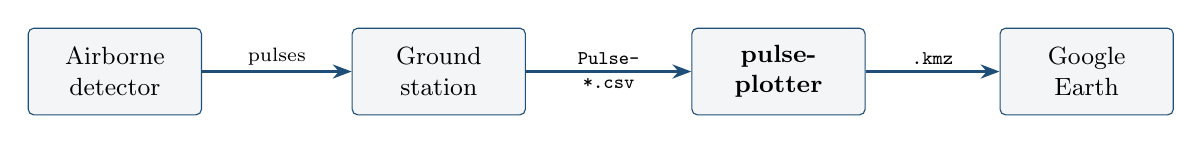
\begin{tikzpicture}[
  box/.style={draw=uavblue,fill=boxgrey,rounded corners=2pt,inner sep=5pt,
              align=center,font=\small,minimum height=11mm,minimum width=22mm},
  lbl/.style={font=\scriptsize,align=center,inner sep=2pt},
  arr/.style={-{Stealth[length=2.4mm]},draw=uavblue,thick}]
\node[box] (air) {Airborne\\detector};
\node[box,right=19mm of air] (gcs) {Ground\\station};
\node[box,right=21mm of gcs] (pp) {\textbf{pulse-}\\\textbf{plotter}};
\node[box,right=17mm of pp] (ge) {Google\\Earth};
\draw[arr] (air) -- node[lbl,above]{pulses} (gcs);
\draw[arr] (gcs) -- node[lbl,above]{\texttt{Pulse-}}
                    node[lbl,below]{\texttt{*.csv}} (pp);
\draw[arr] (pp) -- node[lbl,above]{\texttt{.kmz}} (ge);
\end{tikzpicture}
\end{center}

\noindent The airborne detector is \code{uavrt\_detection} or
\code{MavlinkTagController2}; the ground station is \code{TagTracker}. This
tool does four things:

\begin{enumerate}
\item Reads any of the four pulse-log formats \textsf{TagTracker} has shipped.
\item Plots each pulse at the position the aircraft held when it was received,
      coloured by a property you choose, over an interpolated surface.
\item Estimates a bearing from the aircraft to the tag, with a confidence figure.
\item Exports the whole thing as a self-contained KMZ.
\end{enumerate}

There are two implementations. They are the same tool: same inputs, same
outputs, same numbers. Use whichever suits you.

\begin{center}\small
\begin{tabular}{@{}lll@{}}
\toprule
 & \code{matlab/} & \code{python/} \\
\midrule
Run it        & \code{clear classes; pulseplotter2} & \code{python pulseplotter.py} \\
Needs         & MATLAB, base install, no toolboxes  & Python 3.8+, numpy, matplotlib \\
Licence cost  & MATLAB licence                      & none \\
\bottomrule
\end{tabular}
\end{center}

%======================================================================
\section{Getting started}

\subsection{Python, no MATLAB licence needed}

You need Python 3.8 or newer \emph{with Tk 8.6 or newer}. Check first, because
Apple's system Tk is 8.5.9 and the window will come up almost empty with no
error:

\begin{quote}\code{python3 -c "import tkinter; print(tkinter.TkVersion)"}\end{quote}

\noindent If that prints \code{8.5}, install a Python that bundles Tk 8.6
(\code{brew install python@3.12 python-tk@3.12}, or the python.org installer)
and build the environment from it \emph{by full path}. Then:

\begin{quote}
\code{cd python}\\
\code{python3 -m venv .venv \&\& source .venv/bin/activate}\\
\code{python -m pip install -r requirements.txt}\\
\code{python pulseplotter.py}
\end{quote}

\noindent On Windows the middle two lines are \code{py -m venv .venv} and
\code{.venv\textbackslash Scripts\textbackslash activate}. Every new terminal
needs the activate step again. You can pass a log on the command line to open it
straight away.

\subsection{MATLAB}

\begin{quote}
\code{cd matlab}\\
\code{clear classes}\qquad\% MATLAB caches classdefs --- do not skip this after an edit\\
\code{pulseplotter2}
\end{quote}

\noindent Run \code{pulseplotter2}, not the \code{.mlapp}. The four helper files
(\code{readpulsetable.m}, \code{geo2enu.m}, \code{enu2geo.m}, \code{kmzwrite.m})
must sit in the same folder --- the app calls them by name.

%======================================================================
\section{The pulse log}

One file, one flight. Each row is one detected pulse, carrying the tag it
belongs to, when it arrived, how strong it was, and where the aircraft was.

\textsf{TagTracker} has shipped four header variants of this file, including a
2023 build with no header at all. In every one of them the first sixteen fields
are in the same order and columns 14, 15 and 16 are latitude, longitude and
altitude. The reader therefore parses \emph{positionally} and ignores what the
header calls things, so every variant loads without you having to know which
build wrote it.

Two things it handles that a naive CSV reader does not:

\begin{itemize}
\item The leading \code{\#} on the header line. You do not need to delete it.
\item The four-field rotation start/stop records interleaved among the pulses.
      Read naively these become bogus ``pulses'' carrying a latitude in the
      \code{tag\_id} column, which corrupts the tag list and the plot origin.
\end{itemize}

\noindent The two logs used throughout this guide are real flights from the
November 2025 Cumbria campaign:

\begin{center}\small
\begin{tabular}{@{}llrrl@{}}
\toprule
Flight & File & Pulses & Duration & Tags \\
\midrule
Day 5, 21 Nov & \code{Pulse-2025-11-21-11-08-41-149.csv} & 1111 & 13.3 min & 40, 41, 42, 43 \\
Day 8, 24 Nov & \code{Pulse-2025-11-24-15-42-40-343.csv} &  460 & 10.5 min & 10, 12, 13 \\
\bottomrule
\end{tabular}
\end{center}

%======================================================================
\section{A worked example}

\subsection{Load a flight}

Press \textbf{Load Data} and choose \code{Pulse-2025-11-21-11-08-41-149.csv}.
The plot appears immediately --- there is no separate ``plot'' button. The
\textbf{Tag ID} list fills with the tags present in the file and selects the
most common one.

\begin{figure}[htbp]
\centering
\screenshot{screen-window.png}{0.95\textwidth}
  {The whole window with the Day 5 log loaded.}
\caption{The application window. The control column is on the left, the plot and
its two range sliders on the right. Both implementations use the same
arrangement and the same four control groups.}
\end{figure}

\subsection{Pick a tag}

This flight carried four tags. Changing \textbf{Tag ID} replots for that tag
alone; the grey dots stay put and show every pulse in the file, so you can see
how much of the flight the selected tag actually covers.

\begin{figure}[htbp]
\centering
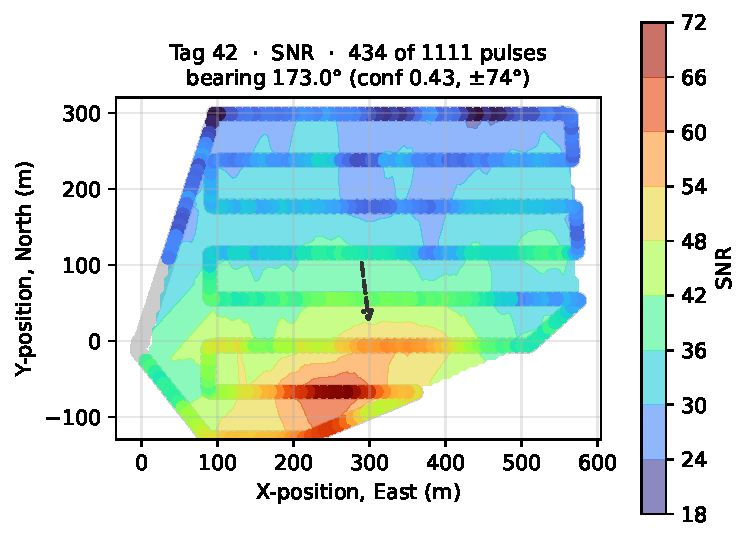
\includegraphics[width=0.49\textwidth]{plot-day5-tag42.pdf}\hfill
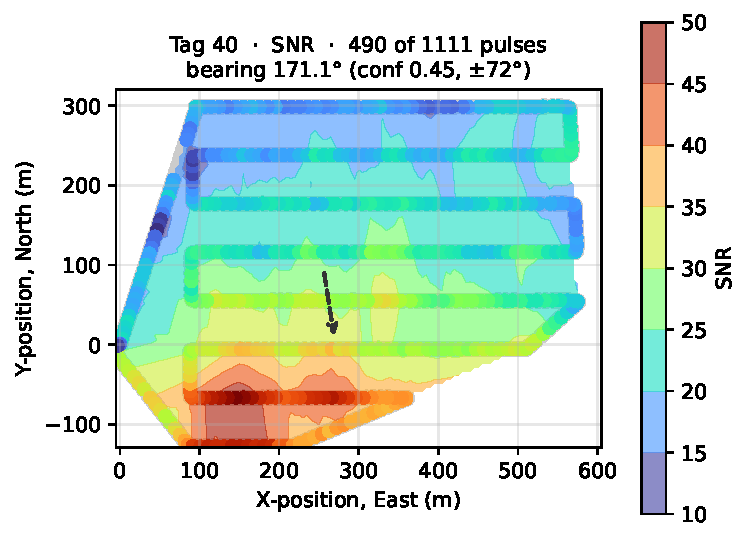
\includegraphics[width=0.49\textwidth]{plot-day5-tag40.pdf}
\caption{Day 5, tag 42 (left, 520 pulses) and tag 40 (right, 490 pulses) from
the same flight. Grey dots are all 1111 pulses; coloured dots are the selected
tag; the filled surface is SNR interpolated over the area flown. Both tags put
the strong signal to the south-east and give bearings within three degrees of
each other. Real output from the application.}
\end{figure}

\subsection{Narrow the selection}

The two range sliders under the plot cut the data down by time and by SNR. Each
is a lower and an upper bound; the plot redraws when you release the handle, not
while you drag. Use the time slider to isolate one leg of the survey, and the
SNR slider to drop noise-floor detections that would otherwise flatten the
surface.

\subsection{Choose what to plot}

\textbf{Property} selects what colours the dots and drives the surface: SNR,
STFT score, time, or altitude. \textbf{Axis} switches between local metres and
degrees. \textbf{Plot Property} switches the surface between the interpolated
value and its divergence, which highlights where the field converges.

\begin{figure}[htbp]
\centering
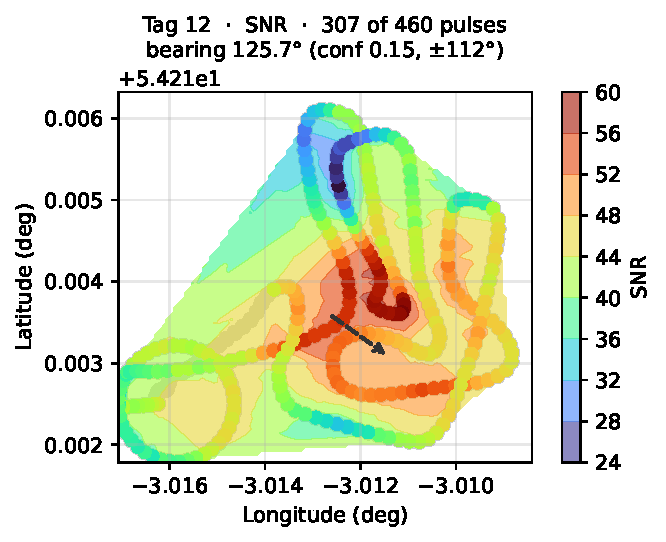
\includegraphics[width=0.49\textwidth]{plot-day8-lonlat.pdf}\hfill
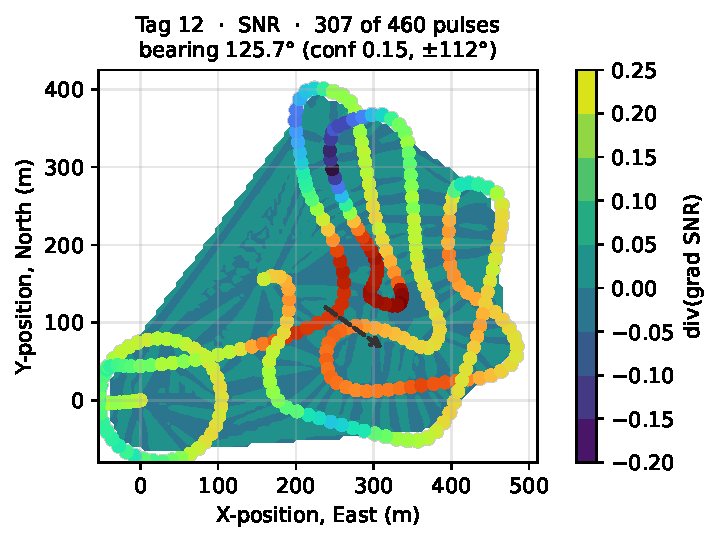
\includegraphics[width=0.49\textwidth]{plot-day8-divergence.pdf}
\caption{Day 8, tag 12. Left: the same data in \code{Lon, Lat} rather than
\code{x, y}; the aspect ratio is corrected for latitude so the map is not
stretched east--west. Right: \textbf{Divergence} mode, which shows where the
gradient field converges --- the dark region is where the surface peaks.}
\end{figure}

\subsection{Export}

\textbf{Export KMZ} (\textbf{Export KML} in MATLAB) writes a single
self-contained archive. Set \textbf{Elev (m)} to the takeoff elevation in metres
MSL first, if you want the pulse markers at their true absolute altitude.

%======================================================================
\section{Controls}

\begin{center}\small
\begin{tabular}{@{}p{0.24\textwidth}p{0.70\textwidth}@{}}
\toprule
\textbf{Data selection} & \\
Tag ID        & Which tag to analyse. Defaults to the most common one in the file. \\
Axis          & Local metres (\code{x, y}) or degrees (\code{Lon, Lat}). \\
Property      & What to colour and contour: SNR, STFT Score, Time, Altitude (m). \\
Start/End Time & The current time window, in seconds from the first pulse. Read-only; driven by the time slider. \\
\midrule
\textbf{Surface} & \\
Smoothing     & Moving-mean window over the property, in pulses. 0 or 1 disables it. \\
Grid Res. (m) & Interpolation grid spacing. Coarsened automatically if a fine grid over a long flight would be too slow. \\
Elev (m)      & Takeoff elevation, metres MSL. Added to the relative pulse altitudes when writing KML. \\
Plot          & Show the interpolated value, or its divergence. \\
\midrule
\textbf{Tag position} & \\
Tag Lat / Lon & A known tag position, for comparison. \\
Plot Tag      & Draw it on the plot and include it in the export. \\
\midrule
\textbf{Bearing} & \\
Active        & Which of the three save slots is live; \textbf{Off} disables saving. \\
Save / Clear  & Store the current bearing in that slot, or empty it. Saved bearings are drawn as solid arrows, the current one as a dashed arrow, so you can compare segments of a flight. \\
Bearing, Confidence, Spread & The current estimate. See section~\ref{sec:theory}. \\
\midrule
\multicolumn{2}{@{}l}{\textbf{Below the plot}} \\
Time / SNR sliders & Lower and upper bounds. Replot on release. \\
\bottomrule
\end{tabular}
\end{center}

\noindent Loading a new file clears all three saved bearing slots: they belong
to the flight they were measured on.

%======================================================================
\section{How the bearing is computed}
\label{sec:theory}

\subsection{The idea}

Received signal strength falls off with distance from the transmitter. If that
is the dominant effect over the area you flew, then the interpolated SNR surface
slopes upward towards the tag, and its gradient points at it. The estimator
takes the gradient everywhere on the grid and asks what direction those arrows
agree on.

\subsection{Local frame}

Pulse positions arrive as latitude, longitude and relative altitude. They are
converted to a local east--north--up frame anchored on the first pulse of the
flight, $(\varphi_0,\lambda_0)$, using the WGS84 meridional and normal radii of
curvature evaluated at that latitude:
%
\begin{equation}
R_M = \frac{a(1-e^2)}{\left(1-e^2\sin^2\varphi_0\right)^{3/2}},
\qquad
R_N = \frac{a}{\sqrt{1-e^2\sin^2\varphi_0}},
\end{equation}
%
\begin{equation}
x_i = (\lambda_i-\lambda_0)\,\frac{\pi}{180}\,R_N\cos\varphi_0,
\qquad
y_i = (\varphi_i-\varphi_0)\,\frac{\pi}{180}\,R_M .
\end{equation}
%
This flat-earth approximation agrees with a rigorous ECEF-based transform to
better than 5\,cm over a 1\,km box. Because it is
linear in $x$ and $y$ independently, a rectangular grid in this frame maps to an
exactly rectangular latitude/longitude box --- which is what lets the KML ground
overlay be exact rather than approximate.

\subsection{Surface}

Let $P_i$ be the chosen property at pulse $i$, optionally replaced by a centred
moving mean over $w$ consecutive pulses. The scattered values are interpolated
onto a regular grid of spacing $\Delta$ by linear interpolation over a Delaunay
triangulation, giving $\hat P_k$ at cell $k$. Cells outside the convex hull of
the flown positions are left undefined and take no part in anything that
follows --- this is also why the exported overlay is transparent there.

\subsection{Resultant}

Central differences give the gradient $\nabla \hat P_k = (F_{x,k}, F_{y,k})$ at
each cell. Let $\mathcal{K}$ be the cells where both components are finite and
the gradient is non-zero. The estimator forms the magnitude-weighted circular
mean of the gradient directions: with unit directions
$\hat u_k = \nabla \hat P_k / \lVert \nabla \hat P_k \rVert$ and weights
$w_k = \lVert \nabla \hat P_k \rVert$,
%
\begin{equation}
\mathbf{R} \;=\; \sum_{k \in \mathcal{K}} w_k \hat u_k
           \;=\; \sum_{k \in \mathcal{K}} \nabla \hat P_k,
\qquad
W \;=\; \sum_{k \in \mathcal{K}} \bigl\lVert \nabla \hat P_k \bigr\rVert .
\label{eq:resultant}
\end{equation}
%
The direction of $\mathbf{R}$ is reported as a compass bearing --- zero at
north, increasing clockwise --- and its normalised length as a confidence:
%
\begin{align}
\theta &= \operatorname{atan2}(R_y, R_x), &
\beta  &= \left(90^\circ - \theta\right) \bmod 360^\circ, \\[2pt]
R      &= \min\!\left(\frac{\lVert \mathbf{R} \rVert}{W},\, 1\right), &
\sigma &= \sqrt{-2\ln R} \quad \text{(radians)} .
\end{align}
%
$\sigma$ is the circular standard deviation implied by a resultant length $R$,
and is the $\pm$ figure in the plot title.

\paragraph{What the weighting does, and does not, do.}
The two forms in equation~\eqref{eq:resultant} are equal, because the weight
$w_k$ cancels the normalisation in $\hat u_k$. The reported \emph{direction} is
therefore exactly the direction of the plain vector sum of the gradient field,
identical to what averaging the components would give. What the circular framing
contributes is $R$ and $\sigma$: the ratio of the length of the summed vector to
the sum of the lengths, which is a genuine measure of how much the field agrees
and has no counterpart in a component average.

\begin{figure}[htbp]
\centering
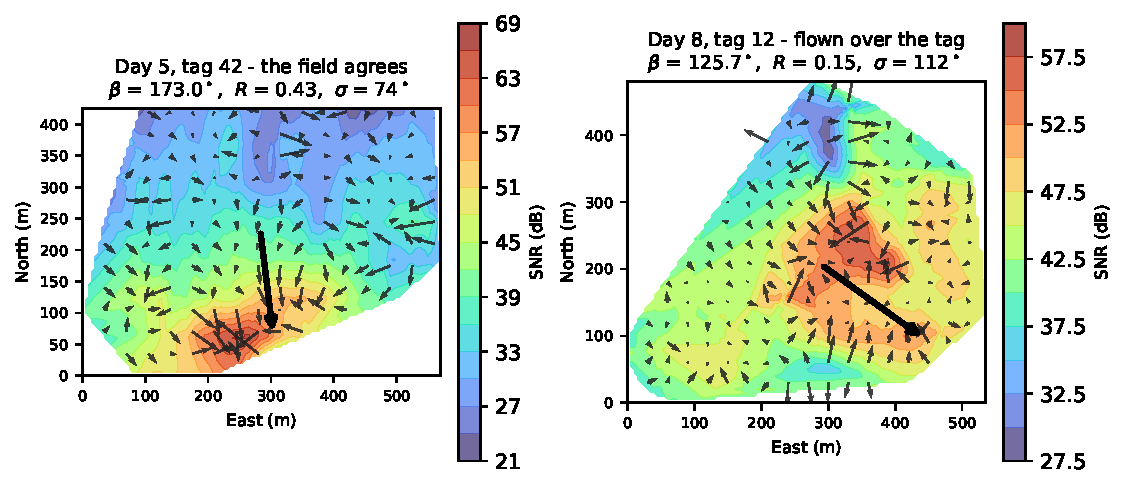
\includegraphics[width=\textwidth]{theory-gradient.pdf}
\caption{The gradient field the estimate is built from, on two real flights.
Left: the arrows broadly agree and the resultant is meaningful. Right: the
aircraft passed over the tag, so the gradients converge on an interior maximum
and cancel; the resultant still has a direction but $R=0.12$ says not to trust
it. Both panels are computed by the application's own code.}
\label{fig:gradient}
\end{figure}

\subsection{Reading the confidence}

$R$ runs from 0 to 1 and measures how much the cells of the field agree on a
direction, not how far the answer is from the truth. It is sensitive: a small
amount of scatter on the surface pulls it down sharply while the bearing itself
is still good, because independent noise in the gradient largely cancels when
summed over thousands of cells.

\begin{figure}[htbp]
\centering
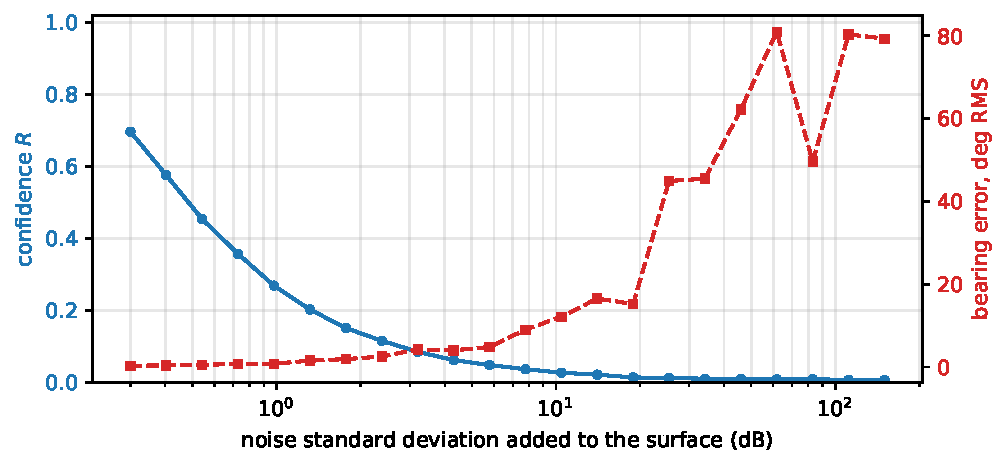
\includegraphics[width=0.86\textwidth]{theory-confidence.pdf}
\caption{A clean planar surface at $45^\circ$ with increasing zero-mean noise.
$R$ has already fallen below 0.2 while the bearing is still within a couple of
degrees. Treat a low $R$ as a warning to look at the plot, not as an error bar.}
\end{figure}

\noindent In practice:

\begin{itemize}
\item \textbf{$R$ above about 0.4} --- the field agrees over most of the area.
      The bearing is worth using.
\item \textbf{$R$ between 0.1 and 0.4} --- partial agreement. Look at the
      surface before believing the number. Often the flight only sampled one
      side of the gradient.
\item \textbf{$R$ below 0.1} --- no consensus. Usually one of the failure modes
      below rather than a noisy but usable estimate.
\end{itemize}

\subsection{When it does not work}

The method assumes the surface slopes monotonically towards the tag across the
area flown. Three things break that assumption:

\begin{description}[style=unboxed,leftmargin=0pt,font=\bfseries]
\item[You flew over the tag.] The surface then has an interior maximum and the
      gradients point inwards from all sides, cancelling --- the right-hand
      panel of figure~\ref{fig:gradient}. This is a good outcome for
      localisation and a useless one for bearing. \textbf{Divergence} mode makes
      it obvious.
\item[Terrain.] Known from field experience: where there is significant
      topography near the aircraft the peak signal can occur slightly downhill
      of the tag rather than above it, and the gradient no longer points at it.
      Prefer the directional antenna and triangulation where terrain is a factor.
\item[You picked a property that is not signal strength.] The estimator will
      happily report a bearing for \textbf{Time} or \textbf{Altitude (m)}, and
      it will be the direction the aircraft climbed or flew, not the direction
      of a tag. Only SNR --- and to a lesser extent STFT score --- carries
      bearing information.
\end{description}

\begin{figure}[htbp]
\centering
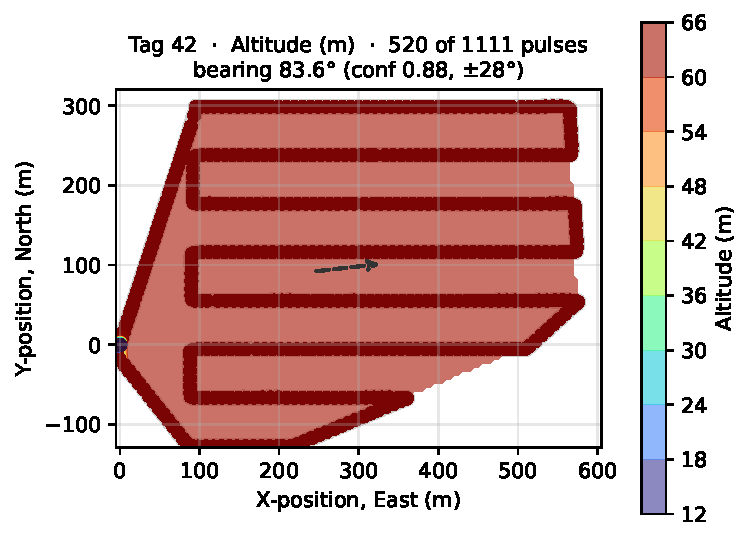
\includegraphics[width=0.52\textwidth]{plot-day5-altitude.pdf}
\caption{The third failure mode, and the reason the confidence is not a measure
of correctness. This is the Day 5 flight with \textbf{Property} set to
\textbf{Altitude (m)}: the surface is the aircraft's own height profile, so the
field agrees strongly ($R=0.88$, the highest number in this guide) on a bearing
of $83.6^\circ$ that has nothing whatever to do with the tag. A high $R$ means
the cells agree, not that you asked a sensible question.}
\end{figure}

\begin{center}
\fcolorbox{rulegrey}{boxgrey}{\begin{minipage}{0.93\textwidth}\small
\textbf{Not yet validated against ground truth.} The estimator is verified
numerically --- exact on clean linear fields, $45.00^\circ$ on a point-source
field whose true bearing is $45^\circ$, with $R$ collapsing as noise rises --- but
it has not been checked against a flight with an independently known tag
position. Treat bearings as indicative.
\end{minipage}}
\end{center}

%======================================================================
\section{The exported KMZ}

One archive, three folders, no network needed --- every icon and image is
packaged inside, so it renders correctly in the field with no connection:

\begin{itemize}
\item \textbf{$\langle$property$\rangle$ surface} --- the interpolated field as
      a semi-transparent raster, transparent outside the area actually flown.
\item \textbf{Contour lines} --- level curves, switched off by default.
\item \textbf{Pulses (tag $N$)} --- one marker per pulse, coloured by the
      property, with the value in its balloon.
\end{itemize}

\noindent If \textbf{Plot Tag} is on, the known tag position is included as a
fourth folder.

%======================================================================
\section{If something goes wrong}

\begin{center}\small
\begin{tabular}{@{}p{0.42\textwidth}p{0.52\textwidth}@{}}
\toprule
Symptom & Cause \\
\midrule
Python: window opens nearly empty, no error &
  Tk 8.5. Rebuild the environment on a Python with Tk 8.6. \\
MATLAB: your edit had no effect &
  MATLAB cached the classdef. \code{clear classes} and rerun. \\
MATLAB: edits to the \code{.mlapp} keep reverting &
  App Designer holds its own copy and writes it back. Edit \code{pulseplotter2.m}. \\
Tag list contains a number that looks like a latitude &
  A rotation record was read as a pulse. Should not happen with this reader; report the log. \\
No surface, only dots &
  Fewer than four finite values, or every value identical, for the selected tag and window. \\
Bearing reads \code{-} &
  No surface, so no gradient. Widen the time or SNR window. \\
The plot crawls on a long flight &
  Grid resolution too fine. It is capped automatically, but a coarser value replots faster. \\
\bottomrule
\end{tabular}
\end{center}

%======================================================================
\appendix
\section{Differences between the two implementations}

The numbers are the same. The differences are all in the interface:

\begin{itemize}
\item The time and SNR ranges are two separate sliders each in Python, rather
      than one two-handled slider; Tk has no native range widget. Their bounds
      are printed beside them, where MATLAB has read-only Start Time and End
      Time fields in the control column.
\item Python includes a matplotlib toolbar, so you can zoom and pan. MATLAB
      cannot.
\item \textbf{Plot Tag} is a checkbox in Python, a slider switch in MATLAB.
\item Python's export writes the KMZ directly; MATLAB goes through a temporary
      \code{.kml}.
\item \code{MONOPOLE\_SCAN\_MAPPING.m}, a standalone antenna-pattern analysis
      script, is MATLAB-only and is not part of the plotter.
\end{itemize}

\noindent Neither has been run side by side on the same log and compared
numerically. That is the obvious next check; until it is done, ``same numbers''
is an intention rather than a measurement.

\section{Reproducing the figures}

Every plot in this guide is real output from the application, generated by
driving the same controls a user would:

\begin{quote}
\code{cd DOCS}\\
\code{../python/.venv/bin/python make\_figures.py}\\
\code{latexmk -pdf pulseplotter-guide.tex}
\end{quote}

\noindent The two pulse logs live outside the repository, under
\code{FLIGHT\_TESTING\_DATA}; pass other paths as arguments if yours are
elsewhere.

\vspace{0.6cm}
\noindent\textcolor{rulegrey}{\rule{\textwidth}{0.8pt}}\\[4pt]
{\small Developed under NSF awards 1556417 and 2104570. Source, licence (GPL-3.0)
and working notes: \code{uavrt\_postflight}.}

\end{document}
